\chapter{Results and discussion}\label{ch:results}
%%%%%%%%%%%%%%%%
%- Introduction of what we are looking for, reminder of hypothesis
%%%%%%%%%%%%%%%%
This chapter explains the experimental data using the methods introduced in the previous chapter. For the X-ray pump-- X-ray probe study, data on heterogeneous clusters, i.e. helium droplets doped with xenon, have been taken at different time delays $\Delta t$. To complement the data, pristine data, i.e. helium droplets and xenon droplets individually, have been recorded at different time delays $\Delta t$ and the static case.\\
The chapter is organized as follows. Section \ref{sec:xenon-data} discusses the pristine xenon data and section \ref{sec:helium-data} covers the pristine helium data. Section \ref{sec:helium-xenon-data} shows the proof of principle that tampered layers mitigate radiation damage effects of an enclosed aerosol sample object.
%
%
%
%%%
\section{Pristine xenon pump--probe data}\label{sec:xenon-data}
%%%%%%%%%%%%%%%%%%%%%%%%%%%
%- Presentation of Xe data
%%%%%%%%%%%%%%%%%%%%%%%%%%%
\begin{figure}
	\centering
		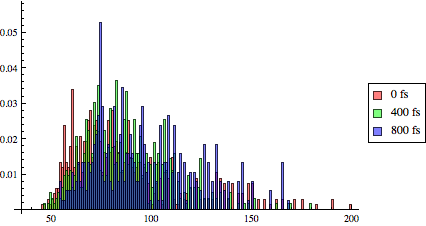
\includegraphics[width=1.00\textwidth]{images/size-distributions.png}
	\caption{caption. MAKE IMAGE NICER}
	\label{fig:size-distributions}
\end{figure}

%
%
%
\subsection{iToF traces with xenon as sample}
- Xe iToF dynamics\\
- Slightly more of Xe higher charge-states present at longer delays.
%
%
%
\subsection{Xenon diffraction images}
- Present study of 1D condensed diffraction images.\\
- Work out similarities to Tais radiation damage
%
%
%
\subsection{Reconstructions of xenon cluster single shot images}
- Present Xe - cluster reconstructions\\
- Show 1D reconstructions and 'damage process'
%
%
%
\subsection{pnCCD image pump -- probe considerations}
- Considerations of pump and probe pulse in one pnCCD image.
%
%
%
\subsection{Time of flight data}
%
%
%
%%%%%%%%%%%%%%%%%%%%%%%%%%%%%%%%%%%%%%%%
\section{Pristine helium cluster pump-probe data}\label{sec:helium-data}
- Presentation of He data
\subsection{iToF data with helium as sample}
- Subsection for iToF data, important to compare to HeXe data.
\subsection{Diffraction images of helium cluster}
- Work out radiation damage in 1D diffraction images.\\
- Introduce envelope to show the radiation damage effect - important to compare to HeXe data.\\
- Eventually subsection for reconstructions.
%
%
%
\section{Helium-xenon core-shell systems and pump--probe data}\label{sec:helium-xenon-data}
-Presentation of HeXe data
\subsection{Time-of-flight data of helium-xenon core-shell systems}
- Show dynamics of XeHe data in tof trace.\\
- More hefty nanoplasma expansion in HeXe than in raw He.\\
- Complement with simulations from Phay.
\subsection{Diffraction images of helium-xenon core shell systems}
- Discuss diffraction images\\
- Show how scattering intensity drops from He signal but not from Xe signal.\\
- Eventually subsection for reconstructions.
\subsection{Core-shell system considerations}
%
%
%
\section{Static data}\label{sec:static}
-Include in other studies? Or appendix?
%
%
%
\section{Conclusion of the X-ray pump -- X-ray probe study}
- Conclusion where the results are compared to each other\\
- This experiment shows that heterogeneous clusters, as in tampered layers, do inhibit radiation damage of the sample target while the sacrificial layer undergoes a rapid nanoplasma transition.